\documentclass{beamer}
\usepackage[utf8]{inputenc}
\usepackage{datetime2}
\usepackage{multicol}
\usepackage{tikz}
\usetikzlibrary{shadows,arrows,fit,matrix,backgrounds}
\usepackage{calc}
\usepackage{booktabs}
\usepackage{makecell}
\usepackage[font=scriptsize]{caption}
\usepackage{csquotes}
\usepackage{xcolor}
\usepackage[ngerman]{babel}
\usetheme{metropolis}
\usepackage[
style=alphabetic,
citestyle=alphabetic,
sorting=nyt]{biblatex}
\addbibresource{literatur.bib}
\setbeamertemplate{frametitle continuation}{\insertcontinuationcount}
% % Definition Progressbar
\makeatletter
\newlength{\custom@progressinheadfoot}
\setbeamertemplate{progress bar in head/foot}{
	\nointerlineskip
	\setlength{\custom@progressinheadfoot}{%
		\paperwidth * \ratio{\insertframenumber pt}{\inserttotalframenumber pt}%
	}%
	\begin{beamercolorbox}[wd=\paperwidth]{progress bar in head/foot}
		\begin{tikzpicture}
		\draw[bg, fill=bg] (0,0) rectangle (\paperwidth, 0.4em);
		\draw[fg, fill=fg] (0,0) rectangle (\custom@progressinheadfoot, 0.4em);
		\end{tikzpicture}%
	\end{beamercolorbox}
}
\addtobeamertemplate{footline}{}{%
	\usebeamertemplate*{progress bar in head/foot}%
}

\tikzset{
    block/.style    = { rectangle, draw=blue, thick, 
	fill=blue!20, text width=4em,
	rounded corners,execute at begin node=\setlength{\baselineskip}{8pt} },
	line/.style     = {draw, thick, ->},
	block2/.style = {block, text width= 6em},
	block3/.style = {block, text width=0.7\textwidth, drop shadow, minimum height=1.5em},
	block4/.style = {block, minimum height=2.2em, drop shadow},
	block5/.style = {block, drop shadow, text centered},
	line2/.style = {line, <->},
}
{
	\tikzset{terminal/.append style={text height=1.5ex,text depth=.25ex}}
	\tikzset{nonterminal/.append style={text height=1.5ex,text depth=.25ex}}
}

\title{12 Factor App}
\subtitle{Eine Methode zur Entwicklung einer Software-as-a-Service (SaaS) Applikation}
\author{Sidney Kuyateh \& Steffen Walter}
\institute{Duale Hochschule Baden-Württemberg}
\date{\today}
\setbeamercolor{progress bar in head/foot}{fg=orange, bg=lightgray}
\begin{document}
	\maketitle
	\AtBeginSection{
		\begin{frame}{Überblick}
			\scriptsize
			\setlength{\baselineskip}{7pt}
			\vspace{0.3cm}
			\tableofcontents[sectionstyle=show, subsectionstyle=show/shaded,currentsection]
		\end{frame}
}
	\begin{frame}{Überblick}
		\scriptsize
		\setlength{\baselineskip}{7pt}
		\vspace{0.3cm}
		\tableofcontents
		\vfill
	\end{frame}
			%%%% Steffen %%%%
		\section{Einführung}
			\metroset{block=fill}
			\subsection{Einführung 12 Factor App und Hintergrund}
				\begin{frame}{Einführung 12 Factor App}
					\begin{block}{Einführung}
						Mit der "12 Factor App" hat Adam Wiggins von der Firma Heroku im Jahr 2011 eine Methode vorgestellt, mit der sich Software-As-A-Service (SaaS) Apps entwerfen und umsetzten lassen, die folgenden Kriterien entsprechen:
						\begin{itemize}
							\item deklarative Formate zur Kosten- und Zeitoptimierung
							\item Klare Schnittstellen zum Betriebssystem für maximale Portabilität
							\item Deploymentmöglichkeiten für modernen Cloudplattformen
							\item Minimierung des Wegs von der Entwicklung zum produktiven Einsatz, für maximale Agilität
							\item Die Möglichkeit zur einfachen Skalierung, ohne weitreichende Änderungen
						\end{itemize}
					\end{block}
				\end{frame}
				\begin{frame}{Hintergrund 12 Factor App}
					\begin{block}{Hintergrund}
						Die Entwickler der 12 Factor App stammen von der Firma Heroku, wo sie der Entwicklung Zahlreicher Webapplikationen im Bereich SaaS beigewohnt haben, um dann die Synthese ihrer Erfahrungen in einem Dokument zu Sammeln und zu Veröffentlichen.\newline
						Das Ziel dabei ist es, dass SaaS Apps künftig einfacher skalierbar sind, besser durch ein Team gepflegt und auf Dauer mit kalkulierbaren Kosten weiterentwickelt werden können. Das Konzept richtet sich gleichermaßen an Entwickler wie auch an Administratoren, die mit dem Deployment betraut sind.
					\end{block}
				\end{frame}
		\section{Die Zwölf Faktoren}
			\subsection{I. Codebase}
				\begin{frame}{I. Codebase}
					\begin{columns}
						\column{0.5\textwidth}
							\begin{itemize}
								\item Versionsmanagementsystem (Git, Subversion, ...)
								\item Codebase - ein Repository (gleicher initialer Commit)
								\item Jede Codebase muss für sich den zwölf Faktoren entsprechen
								\item Eine Duplizierung von Code in verschiedenen Codebases ist nicht zulässig - Bibiliotheken
								\item Eine Codebase - viel Deploys
								\item Jeder Deploy hat die selbe Codebase
							\end{itemize}
						\column{0.5\textwidth}
						\begin{figure}
							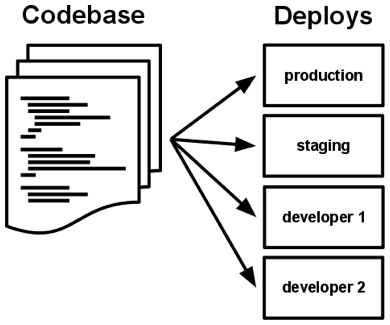
\includegraphics[width=\textwidth]{codebase-deploys.png}
							\caption{Codebasis mit unterschiedlichen Deploymentzweigen \cite{factor-codebase}}
						\end{figure}
					\end{columns}
				\end{frame}
			\subsection{II. Abhängigkeiten}
				\begin{frame}{II. Abhängigkeiten}
					Die meisten Programmiersprachen bieten ein System zur Verwaltung von Bibliotheken an.
					\begin{itemize}
						\item Site Package vs. Bundeling
						\item Abhängigkeitsdeklaration
						\item Isolation von Abhängigkeiten
						\item Systemwerkzeuge (z.B. bash, PowerShell, ...)
					\end{itemize}
				\end{frame}
			\subsection{III. Konfiguration}
				\begin{frame}{III. Konfiguration}
					Konfigurationen dürfen nicht im Quellcode definiert werden. Währende der die App selbst über viele Installationen hinweg statisch ist, unterscheiden sich die Konfigurationen je nach Deploy. Zugangsdaten und Netzwerkadressen sind Beispiele für derartige variable Daten die Ausgelagert werden müssen.
					\begin{itemize}
						\item Konfigurationsdateien (z.B. im yaml Format) - Nachteil: unbestimmter Ort
						\item Umgebungsvariablen - lassen eine klare Trennung von Code und Konfiguration zu und vermeiden Fehler. 
						\item Jeder Zweig der Codebase braucht eigene Umgebung - Nachteil für Skalierbarkeit
					\end{itemize} 
				\end{frame}
			\subsection{IV. Unterstützende Dienste}
				\begin{frame}{IV. Unterstützende Dienste}
					\begin{columns}
					\column{0.5\textwidth}
					Unterstützende Dienste die alle Nachgelagerten Dienste, welche über Netzwerk angesprochen werden. Beispiele für solche Dienste sind Datenbanken, Batchsysteme, Mailing, Cache, uvm.
					\begin{itemize}
						\item On-Premises vs. Cloud Dienste
						\item 
					\end{itemize}
					\column{0.5\textwidth}
					\begin{figure}
						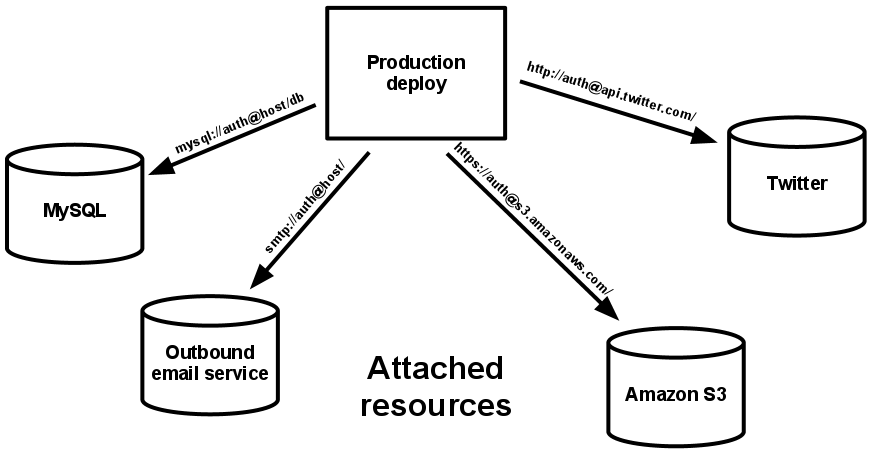
\includegraphics[width=\textwidth]{attached-resources.png}
						\caption{Hintergrunddienste einer Anwendung \cite{factor-subdienst}}
					\end{figure}
					\end{columns}
				\end{frame}
			\subsection{V. Build, Release, Run}
			\subsection{VI. Prozesse}
			%%%% Sidney %%%%
			\subsection{VII. Bindung an Ports}
				\begin{frame}{VII. Bindung an Ports}
					Eine Zwölf-Faktor-App läuft eigenständig und unabhängig von einem gegebenfalls vorhandenem Webserver.
				\begin{itemize}
					\item Verarbeitung von HTTP innerhalb des Appcodes
			 		\item Bindet sich an einen Port und wartet dort auf Requests
					\item Auch andere Protokolle können angeboten werden
				\end{itemize}
			\end{frame}
			\subsection{VIII. Nebenläufigkeit}
			\subsection{IX. Einweggebrauch}
			\subsection{X. Dev-Prod-Vergleichbarkeit}
			\subsection{XI. Logs}
			\subsection{XII. Admin-Prozesse}
		\section{Fazit}
			\subsection{Fazit uns Kritik}
%		\section{Architektursichten}
%		\subsection{Perspektiven}
%			\begin{frame}{Perspektiven}
%				\begin{columns}
%				\column{0.5\textwidth}
%				\begin{itemize}
%					\item Es existiert kein Modell, welches alle relevanten Informationen beinhaltet
%					\item Verschiedene Perspektiven (vgl. \cite{4+1})
%						\begin{itemize}
%						\item Logische Sicht
%						\item Prozessorientierte Sicht
%						\item Entwicklungsorientierte Sicht
%						\item Physische Sicht 
%						\textcolor{gray}{\item Konzeptionelle Sicht}
%						\end{itemize} 
%				\end{itemize}
%			   	\column{0.5\textwidth}
%			   	\begin{figure}
%					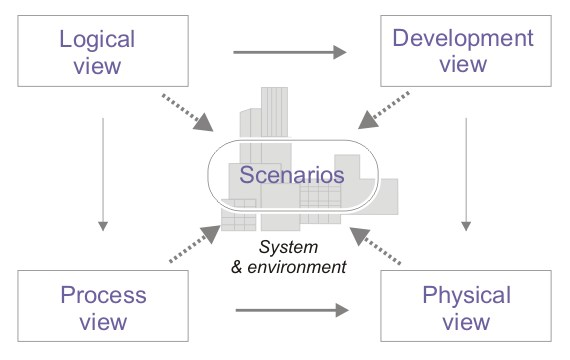
\includegraphics[width=\textwidth]{4+1.jpg}
%					\caption{Darstellung 4+1-Sichtenmodell (vgl. \cite{4+1pic})}
%				\end{figure}
%			\end{columns}
%			\end{frame}
%			\subsection{Notationen}
%			\begin{frame}{Notationen}
%			\begin{columns}
%			\column{0.5\textwidth}
%			\textbf{Informelle Notation (vgl. \cite[ S. 8]{req}}):
%				\begin{itemize}
%					\item Syntax und Semantik nicht oder nur informell vorgegeben
%					\item Beispiel: freie Diagramme
%					\item Vorteilhaft bei der Planung und des Entwurfs von Systemarchitekturen (vgl. \cite[ S. 191]{sommer})
%				\end{itemize}				
%				\column{0.5\textwidth}
%				\textbf{Semi-formale Notation (vgl. \cite[ S. 8]{req}}):
%				\begin{itemize}
%					\item Syntax vorgegeben, Semantik halbformal beschrieben
%					\item Beispiele: UML, OCL
%					\item Vorteilhaft bei der Dokumentation von Systemarchitekturen (vgl. \cite[ S. 191]{sommer})
%				\end{itemize}
%			\end{columns}
%			\textit{Auch existiert die Architectural Description Language (ADL). Nachteil: sehr spezifisch auf das Anwendungfeld zugeschnitten.}
%			\end{frame}
%		
%		\section{Architekturmuster}
%			\subsection{Definition}
%			\begin{frame}{Definition}
%				\begin{block}{Merkmale von Architekturmustern (vgl. \cite{wulff}):}
%					\begin{itemize}
%						\item \enquote{Architekturmuster beschreiben die grundsätzliche 
%						Struktur und Organisation einer Anwendung und 
%						liegen auf der höchsten Abstraktionsebene.}
%					
%						\item \enquote{Ein Architekturmuster beschreibt die Menge 
%						vordefinierter Subsysteme, spezifiziert deren 
%						Zuständigkeit und enthält Regeln zu Organisation 
%						der Beziehungen zwischen ihnen.}
%					
%						\item \enquote{Architekturmuster sind prinzipiell 
%						sprach neutral
%						und Plattform unabhängig.}
%					\end{itemize}
%				\end{block}
%			\end{frame}
%			\subsection{Model-View-Controller-Muster}
%			\begin{frame}[allowframebreaks]{Model-View-Controller-Muster}
%			   	\begin{figure}
%					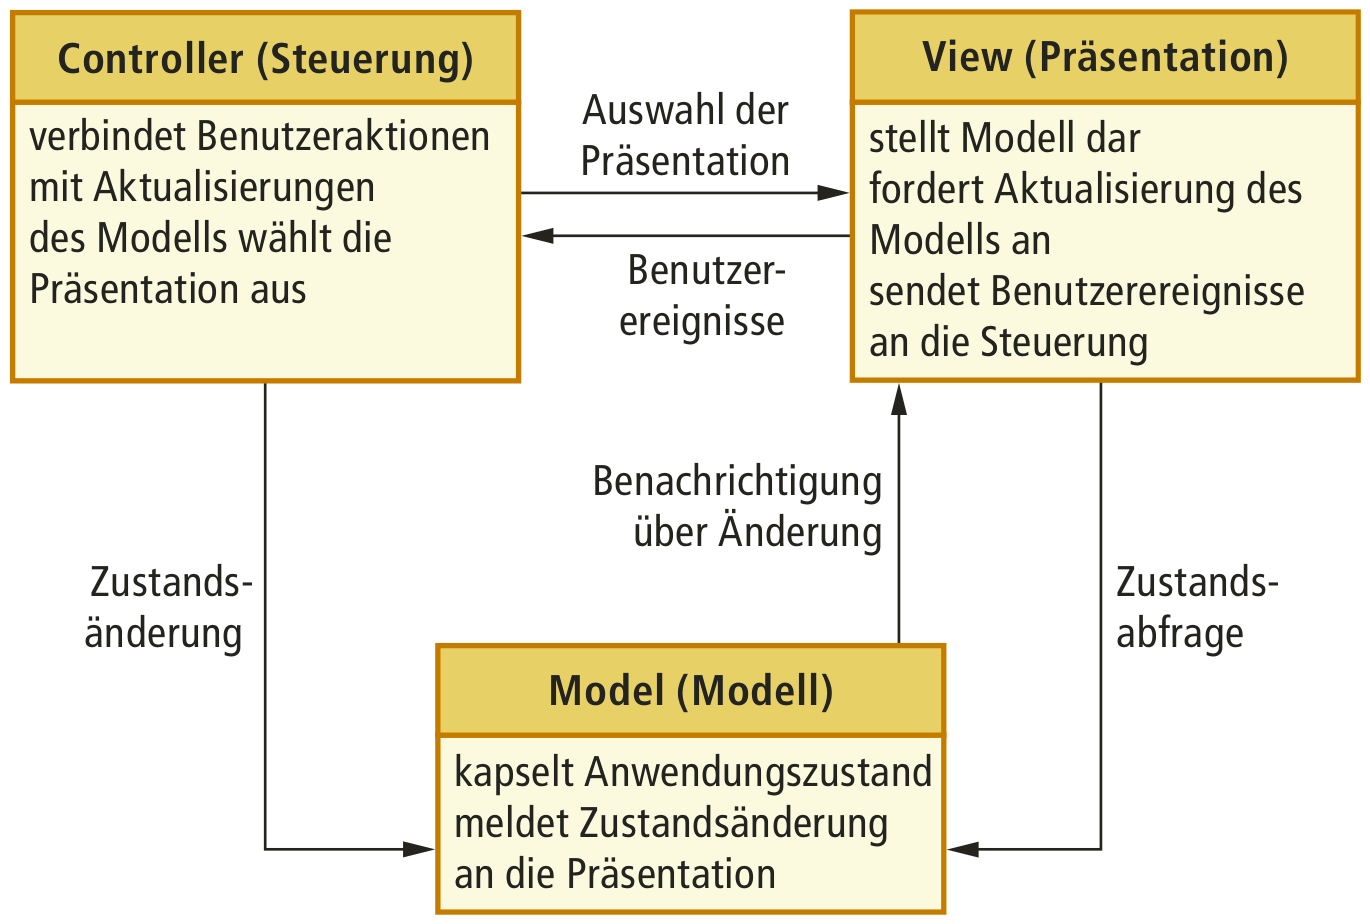
\includegraphics[width=0.8\textwidth]{mvc.png}
%					\caption{Model-View-Controller (MVC) (vgl. \cite[ S.193]{sommer})}
%				\end{figure}
%				\begin{figure}
%					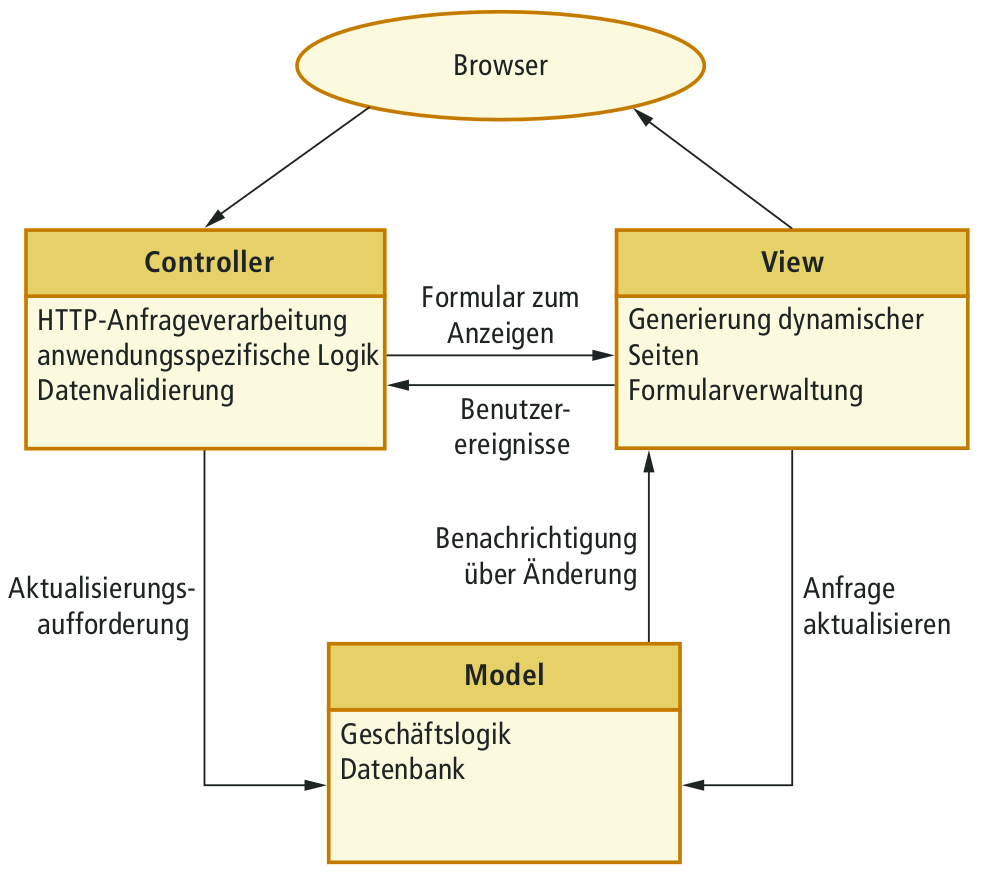
\includegraphics[width=0.6\textwidth]{mvc_bsp.png}
%					\caption{Architektur eine Webanwendung im MVC-Modell (vgl. \cite[ S.193]{sommer})}
%				\end{figure}
%			\end{frame}
%			\subsection{Schichtenarchitektur}
%			\begin{frame}{Schichtenarchitektur (vgl. \cite[ S. 194]{sommer})}
%			\begin{tabular}{*{2}{l}}
%				\toprule
%				\textbf{Name}&\textbf{Schichtenarchitektur}\\
%				\midrule
%				\midrule
%				\textbf{Beschreibung}&\makecell[l]{Strukturierung in Schichten und hierarchischer\\ Aufbau von Diensten.}\\
%				\midrule
%				\textbf{Verwendung}&\makecell[l]{Zur Erweiterung von Systemen, der Arbeit in\\ Teams und bei mehreren Sicherheitsebenen.}\\
%				\midrule
%				\textbf{Vorteile}&\makecell[l]{Bei konstanten Schnittstellen können ganze\\ Schichten ausgetauscht werden.\\ Modulare Nutzung ist möglich.}\\
%				\midrule
%				\textbf{Nachteile}&\makecell[l]{Probleme durch klare Trennung von Schichten\\ und Einhaltung der Hierarchie.}\\
%				\bottomrule
%			\end{tabular}
%			\end{frame}
%			\subsection{Repository-Architektur}
%			\begin{frame}{Repository-Architektur (vgl. \cite[ S. 196f]{sommer})}
%			\begin{tabular}{*{2}{l}}
%				\toprule
%				\textbf{Name}&\textbf{Repository-Architektur}\\
%				\midrule
%				\midrule
%				\textbf{Beschreibung}&\makecell[l]{Zentrale Schnittstelle und Datenspeicher ist das\\ Repository. Interaktion zwischen Komponenten\\ läuft ausschließlich über das Repository.}\\
%				\midrule
%				\textbf{Verwendung}&\makecell[l]{Fokus auf lange Speicherung und große Daten-\\mengen.}\\
%				\midrule
%				\textbf{Vorteile}&\makecell[l]{Unabhängigkeit der Komponenten, Systemweite\\ Änderungen durch eine Komponente möglich.}\\
%				\midrule
%				\textbf{Nachteile}&\makecell[l]{Fehler beim Repository wirken sich auf das ganze\\ System aus. Flaschenhals durch zentrale Kom-\\munikationsschnittstelle}\\
%				\bottomrule
%			\end{tabular}
%			\end{frame}	
%			\subsection{Client-Server-Architektur}
%			\begin{frame}{Client-Server-Architektur (vgl. \cite[ S. 198]{sommer})}
%			\begin{tabular}{*{2}{l}}
%				\toprule
%				\textbf{Name}&\textbf{Client-Server-Architektur}\\
%				\midrule\midrule
%				\textbf{Beschreibung}&\makecell[l]{Funktionen werden durch Dienste zur Verfügung\\ gestellt. Jeder Dienst wird durch einen Server\\ bereitgestellt. Clients greifen auf den Server zu\\ um den gewünschten Dienst aufzurufen.}\\\midrule
%				\textbf{Verwendung}&\makecell[l]{Zugriff auf gemeinsame Datenbank möglich. Gute\\ Hardwareauslastung durch serverbasiertes Modell.}\\\midrule
%				\textbf{Vorteile}&\makecell[l]{Verteilung über Netzwerk ist möglich. Grund-\\funktionen können zentral angeboten werden.}\\\midrule
%				\textbf{Nachteile}&\makecell[l]{Angriffe über das Netzwerk sind möglich.\\ Performanceeinbußen durch Netzwerkprotokolle.}\\
%				\bottomrule
%			\end{tabular}
%			\end{frame}	
%	%%%% Sidney %%%%
%	\section{Anwendungsarchitekturen}
%		\subsection{Nutzung von Anwendungsarchitekturen}
%			\begin{frame}{Nutzung von Anwendungsarchitekturen}
%				\begin{itemize}
%					\item Enthalten die Haupteigenschaften einer Systemklasse
%					\item Allgemeine architektonische Struktur kann beibehalten werden für neue Systeme desselben Typs
%					\item Hilfe bei:
%					\begin{itemize}
%						\item Funktion von Anwendungen verstehen
%						\item Anwendungen desselben Typs vergleichen
%						\item Systementwürfe für Anwendungen vergleichen 
%						\item Wiederverwendbarkeit umfangreicher Komponenten einschätzen
%					\end{itemize}
%				\end{itemize}
%			\end{frame}
%		\subsection{Transaktionsverarbeitende Systeme}
%			\begin{frame}{Transaktionsverarbeitende Systeme}
%				\begin{block}{Definition:}
%					\enquote{Das Ziel Transaktionsverarbeitender Systeme (TP) ist die Verarbeitung von Benutzeranfragen nach Informationen aus einer Datenbank oder Anfragen zum Aktualisieren der Datenbank.} \cite[S. 204]{sommer}
%				\end{block}
%				\begin{itemize}
%					\item Alle Schritte der Transaktion müssen abgeschlossen sein, bevor Änderungen in die Datenbank geschrieben werden
%					\item Transaktionsmanager ist für die Kommunikation mit der Datenbank verantwortlich
%				\end{itemize}
%			\begin{figure}
%				\begin{tikzpicture}[text centered]
%				\matrix[ampersand replacement=\&, column sep=4mm] {
%					\node (p1) [block4] {\tiny E/A-Verarbeitung}; \&
%					\node (p2) [block4] {\tiny Anwendungs"-logik}; \&
%					\node (p3) [block4] {\tiny Transaktions"-manager}; \&
%					\node (p4) [block4] {\tiny Datenbank}; \\
%				};
%				\path [line] (p1) -> (p2);
%				\path [line] (p2) -> (p3);
%				\path [line] (p3) -> (p4);
%				\end{tikzpicture}
%				\caption{Die Struktur transaktionsverarbeitender Anwendungen \cite[S. 204]{sommer}}
%			\end{figure}
%			\end{frame}
%		\subsection{Informationssysteme}
%			\begin{frame}{Informationssysteme 1}
%				\begin{itemize}
%					\item Alle Systeme mit einer gemeinsam genutzten Datenbank können als transaktionsbasierte Informationssysteme betrachtet werden (vgl. \cite[S. 205]{sommer})
%					\item Kontrollierter Zugriff auf eine große Informationsbasis
%				\end{itemize}
%				\begin{figure}
%					\begin{tikzpicture}[text centered]
%					\matrix[row sep=2mm] {
%						\node (p1) [block3] {\tiny Benutzerschnittstelle}; \\
%						\node (p2) [block3] {\tiny \begin{tabular}{l r}
%							Benutzerkommunikation & Authentifizierung und Autorisation
%							\end{tabular}
%						}; \\
%						\node (p3) [block3] {\tiny Abrufen und Ändern von Informationen}; \\
%						\node (p4) [block3] {\tiny Transaktionsverwaltung \\ Datenbank}; \\
%					};
%					\end{tikzpicture}
%					\caption{Schichtenarchitektur eines Informationssystems \cite[S. 205]{sommer}}
%				\end{figure}
%			\end{frame}
%		
%			\begin{frame}{Informationssysteme 2}
%				\begin{itemize}
%					\item Heutzutage meist webbasierte Systeme
%					\item Schichten häufig softwaretechnisch aufgeteilt:
%					\begin{itemize}
%						\item Webserver: Benutzerkommunikation
%						\item Anwendungsserver: Anwendungslogik, Abrufen und Ändern von Informationen
%						\item Datenbankserver: Transaktionsmanagement, Ausführen der Datenbankoperationen
%					\end{itemize}
%				\end{itemize}
%			\end{frame}
%			
%		\subsection{Sprachverarbeitende Systeme}
%			\begin{frame}{Sprachverarbeitende Systeme 1}
%				\begin{itemize}
%					\item Übersetzen eine natürliche oder künstliche Sprache in eine andere Darstellung \cite[S. 207]{sommer}
%					\item Beispiele: Compiler, Dateikonverter, Natürliche Übersetzungssysteme
%				\end{itemize}
%				\begin{figure}
%					\begin{tikzpicture}
%						\matrix[ampersand replacement=\&, column sep = 5mm, row sep = 5mm] {
%							\node (p1) [block] {\tiny Anweisungen der Quellsprache}; \& \node (p2) [block2] {\tiny \textbf{Übersetzer:} \\[1em] Syntax prüfen; \\ Semantik prüfen; \\ Erstellen}; \& \\
%							\& \node (p3)  [block2]  {\tiny abstrakte Maschinenanweisungen}; \& \\
%							\node (p4) [block] {\tiny Daten}; \& \node (p5) [block2] {\tiny \textbf{Interpreter:} \\[1em] abrufen; \\ ausführen}; \&
%							\node (p6) [block]  {\tiny Ergebnisse};\\
%						};
%						\path [line] (p1) -> (p2);
%						\path [line] (p2) -> (p3);
%						\path [line] (p3) -> (p5);
%						\path [line] (p4) -> (p5);
%						\path [line] (p5) -> (p6);
%					\end{tikzpicture}
%					\caption{Die Architektur eines sprachverarbeitenden Systems \cite[S. 208]{sommer}}
%				\end{figure}
%			\end{frame}
%	
%			\begin{frame}{Sprachverarbeitende Systeme 2}
%				\begin{itemize}
%					\item Architektur eines Compilers:
%					\begin{itemize}
%						\item lexikalische Analyse
%						\item Symboltabelle
%						\item Syntaxanalyse
%						\item Syntaxbaum
%						\item Semantikanalyse
%						\item Codegenerator
%					\end{itemize}
%				\end{itemize}
%			
%				\begin{figure}
%					\begin{tikzpicture}
%						\matrix[ampersand replacement=\&, column sep = 5mm, row sep = 5mm] {
%							\& \node (p1) [block5] {\tiny
%									Symboltabelle \\
%									Syntaxbaum}; \& \\
%							\node (p2) [block5] {\tiny lexikalische Analyse}; \& \node (p3) [block5] {\tiny syntaktische Analyse}; \& \node (p4) [block5] {\tiny semantische Analyse}; \& \node (p5) [block5] {\tiny Codegenerierung};\\
%						};
%						\path [line2] (p1) -> (p2);
%						\path [line2] (p1) -> (p3);
%						\path [line2] (p1) -> (p4);
%						\path [line2] (p1) -> (p5);
%						\path [line] (p2) -> (p3);
%						\path [line] (p3) -> (p4);
%						\path [line] (p4) -> (p5);
%					\end{tikzpicture}
%					\caption{Pipes-and-Filter-Architektur für einen Compiler \cite[S. 209]{sommer}}
%				\end{figure}
%			\end{frame}
%				
%			\begin{frame}{Sprachverarbeitende Systeme 3}
%				\begin{itemize}
%					\item Problem bei der Pipes-and-Filter-Architektur: Verbindung mit weiteren Werkzeugen nicht möglich
%					\item Effektiver: Repository-Architektur
%				\end{itemize}
%				\begin{figure}
%					\begin{tikzpicture}
%						\matrix (table) [matrix of nodes, nodes in empty cells, ampersand replacement=\&, column sep = 10mm, row sep = 10mm] {
%							  \& \node (p1) [block5] {\tiny lexikalische Analyse}; \& \node [block5] (p2) {\tiny syntaktische Analyse}; \& \node (p3) [block5]  {\tiny semantische Analyse}; \\
%							\node (p4) [block5] {\tiny Textformatierer}; \& \node [block5, minimum height = 1em] (p11) {\tiny abstrakter Syntaxbaum}; \& \node [block, minimum height = 1em] (p12) {\tiny Grammatik\-definition}; \&[-5mm] \node [block5] (p5) {\tiny Optimierer}; \\
%							\node (p6) [block5] {\tiny Editor}; \& \node [block5, minimum height = 1em] (p13) {\tiny Symbol-\\tabelle}; \& \node [block5, minimum height = 1em] (p14) {\tiny Ausgabe\-definition}; \&[-5mm] \node [block5] (p7) {\tiny Codegenerator}; \\
%						};
%						\begin{scope}[on background layer]
%						\node (p10) [fit=(p11)(p12)(p13)(p14),fill=blue!50]{Repository};
%						\end{scope}
%						
%						
%						\path [line2] (p10) -> (p2);
%						\path [line2] (p10) -> (p3);
%						\path [line2] (p10) -> (p4);
%						\path [line2] (p10) -> (p5);
%						\path [line2] (p10) -> (p1);
%						\path [line2] (p10) -> (p6);
%						\path [line2] (p10) -> (p7);
%					\end{tikzpicture}
%					\caption{Repository-Architektur für ein sprachverarbeitendes System \cite[S. 209]{sommer}}
%				\end{figure}
%			\end{frame}

	\begin{frame}[allowframebreaks]
		\frametitle{Quellen}
		\renewcommand{\bibfont}{\scriptsize}
		\printbibliography[heading=none]
	\end{frame}
\end{document}


